\documentclass[letter,12pt]{article}

\usepackage{subfig}

\usepackage[english]{babel}

\usepackage{fancyhdr}


\usepackage{graphicx}
\usepackage{amsmath}
\usepackage{amssymb}
\usepackage[latin1]{inputenc}
\usepackage{fancybox}
\usepackage{amsfonts}
\usepackage{bbold}
\usepackage{textcomp}


\setlength{\oddsidemargin}{0in}
\setlength{\evensidemargin}{0in}
\setlength{\textwidth}{16.1 cm}
\setlength{\topmargin}{-15mm}
\setlength{\textheight}{22cm}
\setlength{\parindent}{0cm}


\newcommand{\sv}{\underline}
\newcommand{\Sig}{\boldsymbol{\sigma}}
\newcommand{\K}{\boldsymbol{K}}
\newcommand{\Eps}{\boldsymbol{\varepsilon}}
\newcommand{\intener}{\mathcal{E}}


% --------------------------------------------------------------------------------------
% - definition des notations
% --------------------------------------------------------------------------------------


% - tenseur d'ordre 4
\newcommand{\TTTT}[1]{\underline{\underline{\underline{\underline{#1}}}}}
% - tenseur d'ordre 2
\newcommand{\TT}[1]{\underline{\underline{#1}}}
% - tenseur d'ordre 1
\newcommand{\T}[1]{\underline{#1}}

% - composante i - j de la contrainte: 
\newcommand{\sigi}[1]{\sigma_{#1}}
% - composante i - j de la deformation: 
\newcommand{\epsi}[1]{\varepsilon_{#1}}

% - tenseur de contrainte : 
\newcommand{\sig}{\TT{\sigma}}
\newcommand{\eps}{\TT{\varepsilon}}
\newcommand{\C}{\TTTT{C}}
\renewcommand{\S}{\TTTT{S}}

% - composantes des tenseurs de Hooke: 
\newcommand{\Ci}[1]{C_{#1}}
\newcommand{\Si}[1]{S_{#1}}

% - notations pour un vecteur
\renewcommand{\Vec}[1]{\underline{#1}}


% - notations pour un vecteur chapeau
\newcommand{\Vecc}[1]{\hat{\underline{#1}}}

% - notations pour un produit tensoriel
\newcommand{\tens}[2]{#1 \otimes #2}

% - notations pour les vecteurs de base
\newcommand{\e}[1]{\Vec{e_{#1}}}

% - contrainte equivalente pour les crit�res de plasticite
\newcommand{\se}{\sigma_{eq}}

% - deformation elastique
\newcommand{\epse}{\TT{\varepsilon_e}}

% - deformation elastique
\newcommand{\epsp}{\TT{\varepsilon_p}}


\begin{document}
\pagestyle{fancy}

\title{ME 211A: Quadratic Transformation}

\maketitle




We consider the transformation  $\T{x}=\T{\Phi}(\T{X},t)$ defined by: 
\begin{eqnarray}
x_1 & = & X_1 + 0.1 X_2^2 + 10 \\ 
x_2 & = &  \beta X_1^2 + X_2 + 10  \\ 
x_3 & = & X_3 
\end{eqnarray}


\noindent\textbf{Question 1:} Calculate the gradient of the transformation? \\

\textbf{Answer 1 :} The gradient of transformation?

\[\underline{\underline{F}}=\left[ \begin{matrix}
{{F}_{11}} & {{F}_{12}} & {{F}_{13}}  \\
{{F}_{21}} & {{F}_{22}} & {{F}_{23}}  \\
{{F}_{31}} & {{F}_{32}} & {{F}_{33}}  \\
\end{matrix} \right]=\frac{\partial \underline{x}}{\partial \underline{X}}=\left[ \begin{matrix}
\frac{\partial {{x}_{1}}}{\partial {{X}_{1}}} & \frac{\partial {{x}_{1}}}{\partial {{X}_{2}}} & \frac{\partial {{x}_{1}}}{\partial {{X}_{3}}}  \\
\frac{\partial {{x}_{2}}}{\partial {{X}_{1}}} & \frac{\partial {{x}_{2}}}{\partial {{X}_{2}}} & \frac{\partial {{x}_{2}}}{\partial {{X}_{3}}}  \\
\frac{\partial {{x}_{3}}}{\partial {{X}_{1}}} & \frac{\partial {{x}_{3}}}{\partial {{X}_{2}}} & \frac{\partial {{x}_{3}}}{\partial {{X}_{3}}}  \\
\end{matrix} \right]=\left[ \begin{matrix}
1 & 0.2{{x}_{2}} & 0  \\
2\beta {{x}_{1}} & 1 & 0  \\
0 & 0 & 1  \\
\end{matrix} \right]\] \\

\newpage
\noindent \textbf{Question 2:} Make a graphical representation of the reference configuration and of the deformed configuration for some specific values ($\beta=0$, $\beta=0.025$, \dots)? \\


\textbf{Answer 2:} We define the original shape as a $10\times10\times10 mm^3$ cube. Fig. \ref{fig:1} (a) gives the original and deformed shape with $\beta=0$. Since the coordinate in the third direction is not changed, we can see it as a 2D deformation problem and make the comparison more clear, like in Fig. \ref{fig:1} (b). Fig. \ref{fig:2} (a)-(d) shows the reference and deformed configuration with $\beta=0, 0.01, 0.025, 0.05$ respectively. \\
\begin{figure}[ht]
	\centering
	\subfloat[][$\beta=0$]{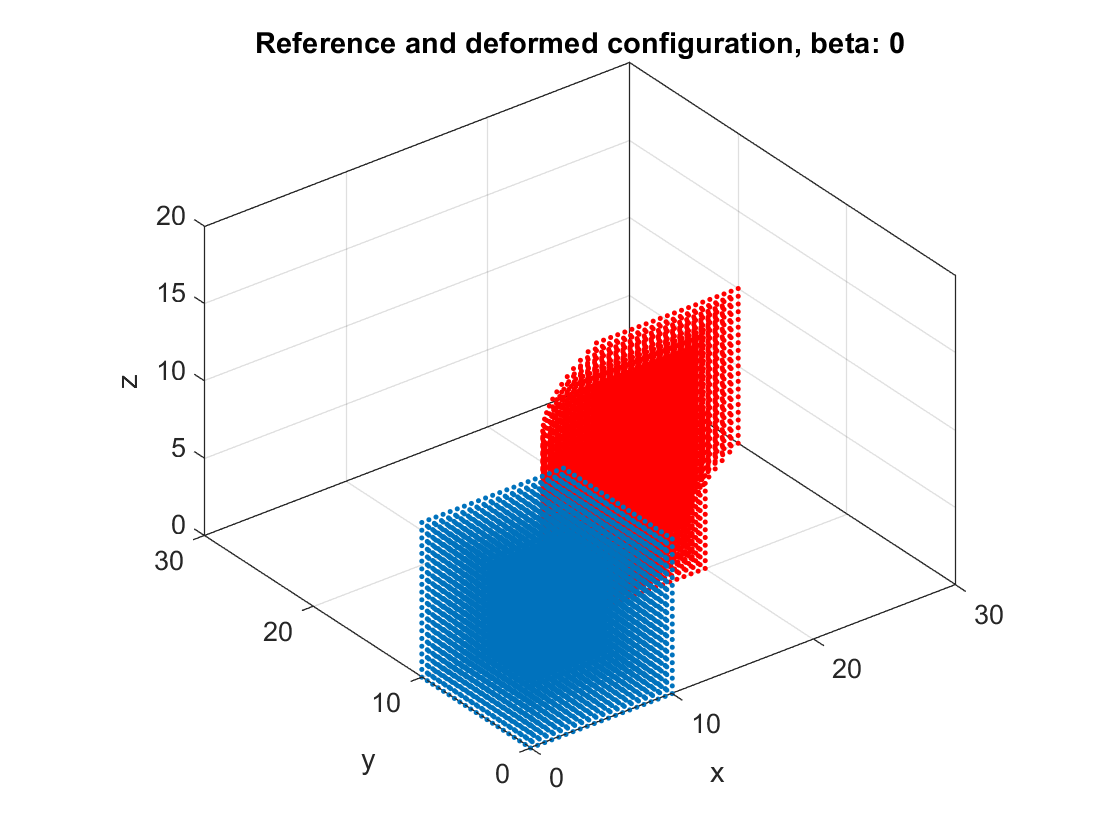
\includegraphics[width=.45\textwidth]{1.png}}\quad
	\subfloat[][$\beta=0$]{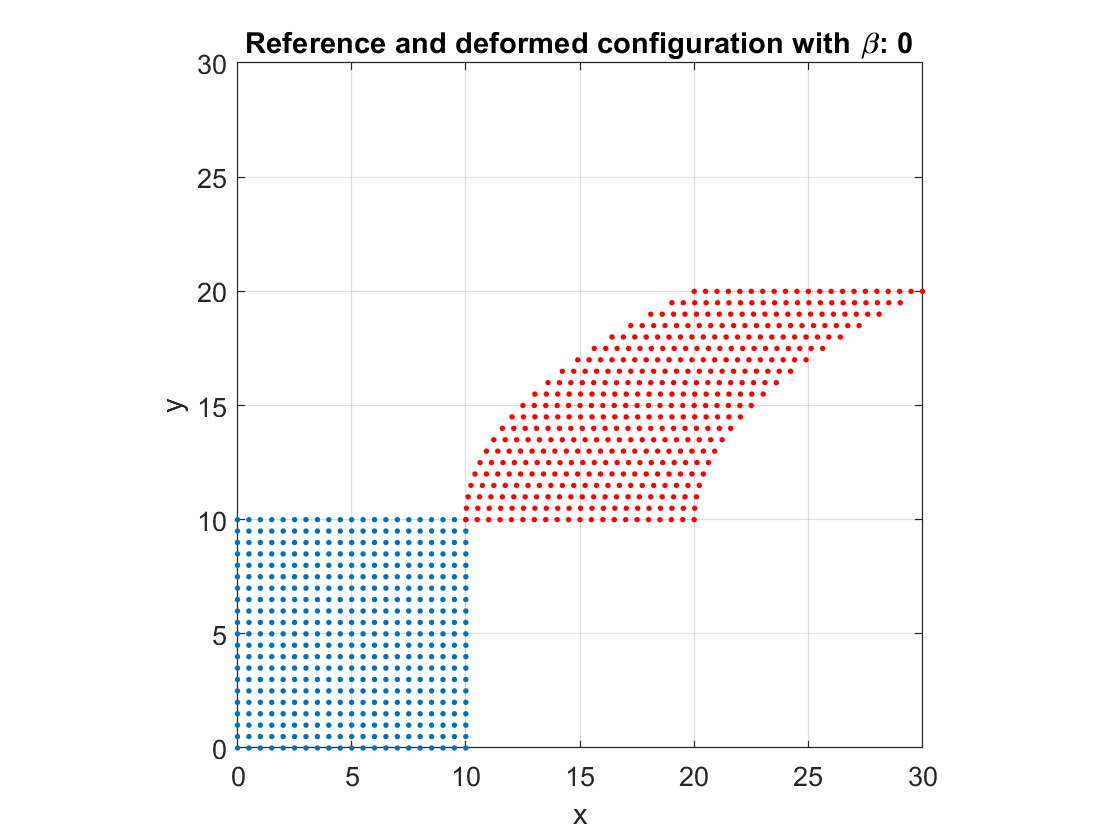
\includegraphics[width=.45\textwidth]{1_1.png}}\quad
	\caption{3D and 2D plot of original and deformed shape at $\beta=0$.}
	\label{fig:1}
\end{figure}

\begin{figure}[ht]
	\centering
	\subfloat[][$\beta=0$]{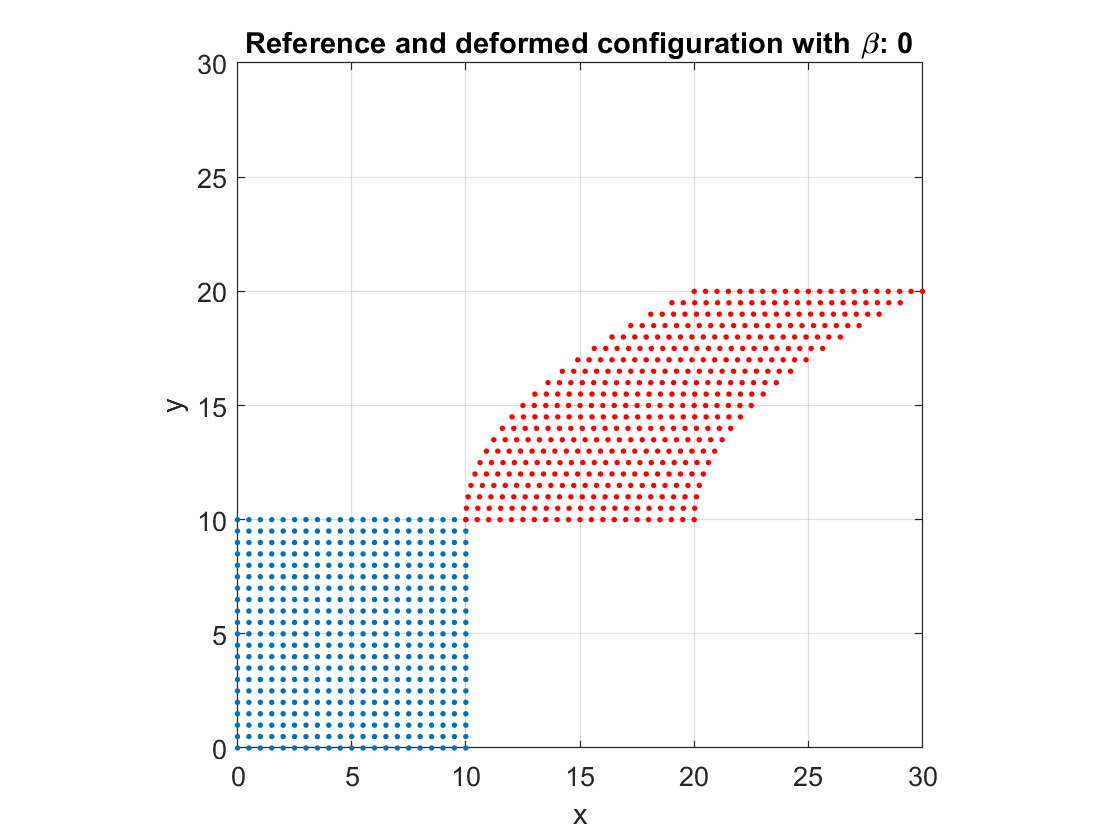
\includegraphics[width=.45\textwidth]{1_1.png}}\quad
	\subfloat[][$\beta=0.01$]{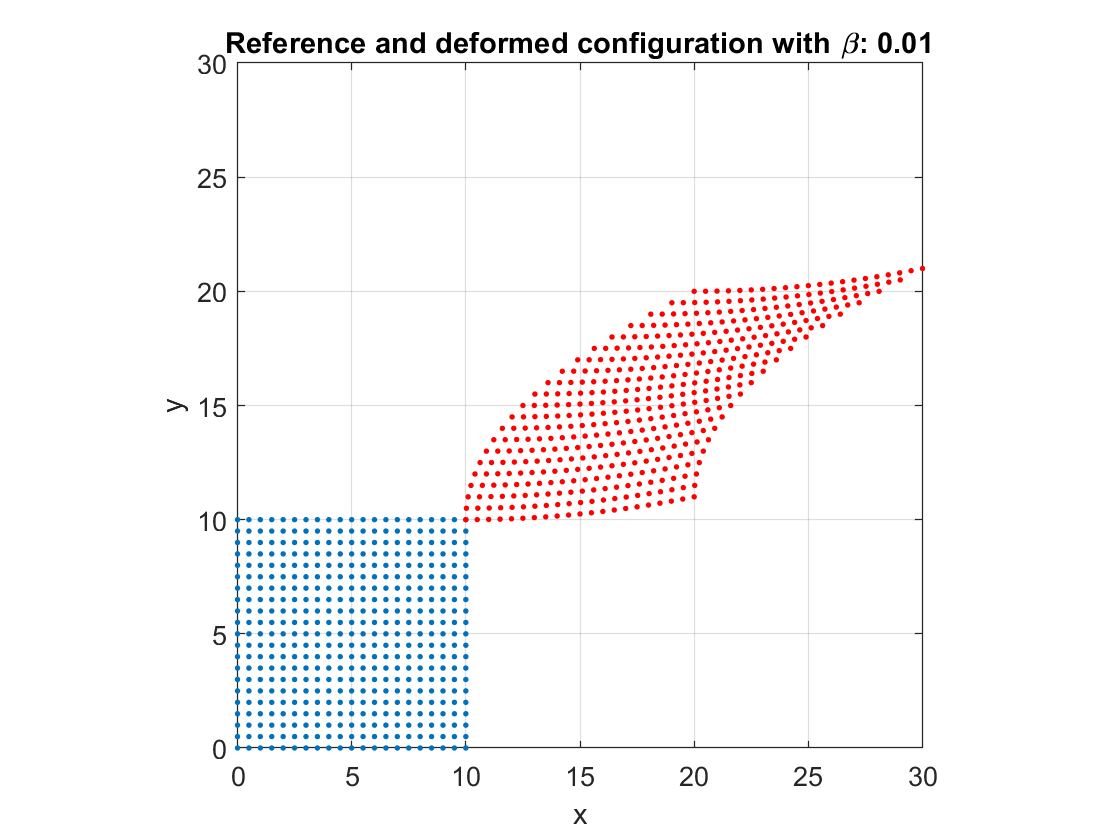
\includegraphics[width=.45\textwidth]{4.png}}\\
	\subfloat[][$\beta=0.025$]{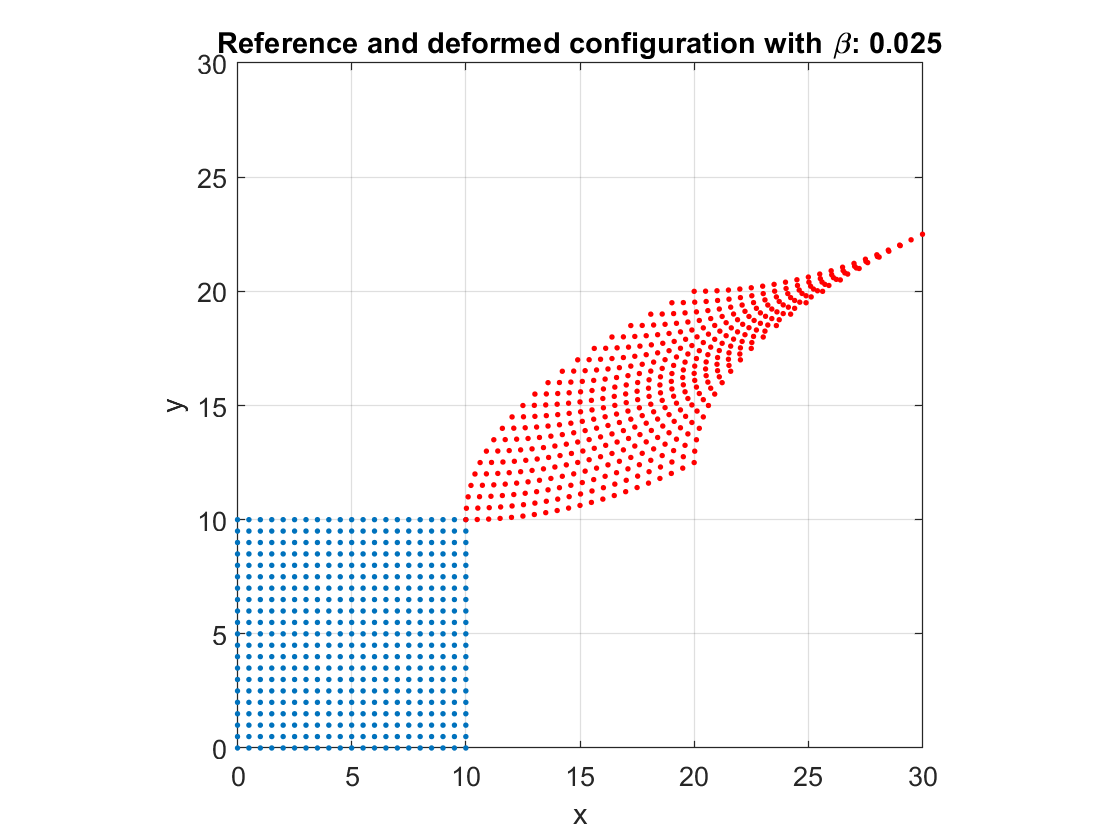
\includegraphics[width=.45\textwidth]{6.png}}\quad
	\subfloat[][$\beta=0.05$]{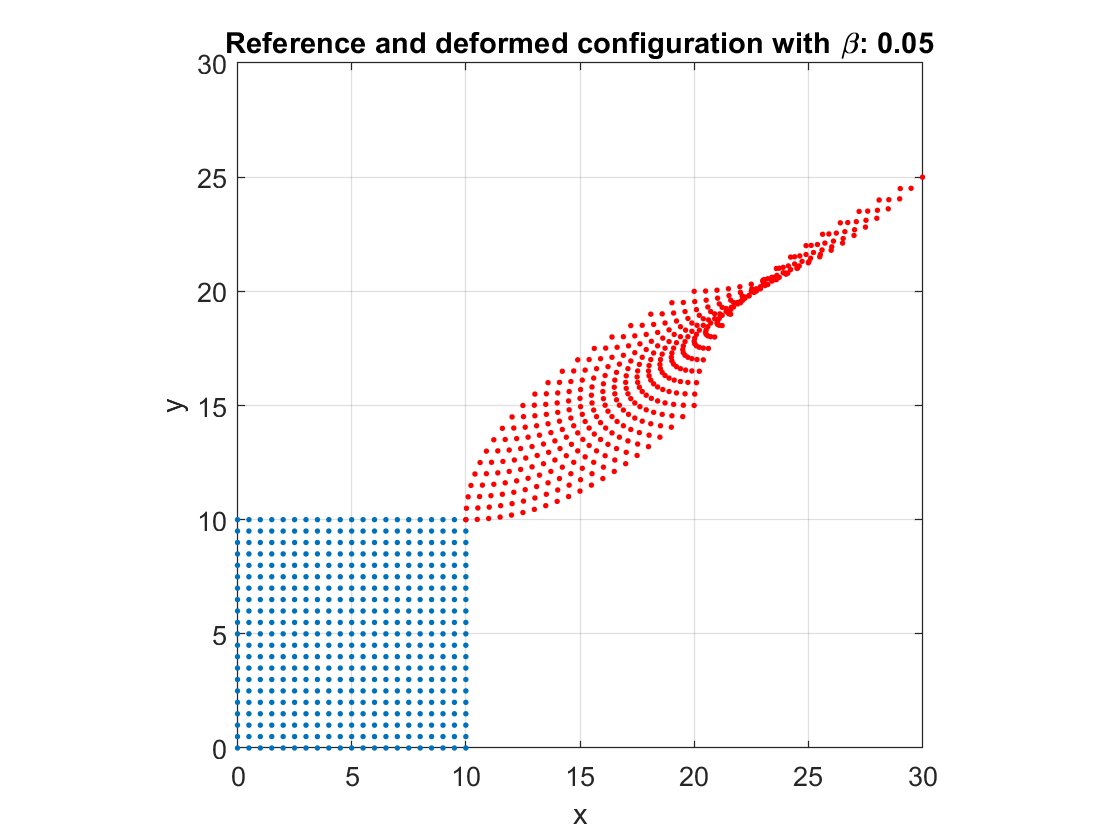
\includegraphics[width=.45\textwidth]{8.png}}
	\caption{2D (x-y) plot of original and deformed shape.}
	\label{fig:2}
\end{figure}

\newpage
\noindent \textbf{Question 3:} What is the value of the local variation of volume? \\

\textbf{Answer 3:} The local variation of volume is the determinant of $\underline{\underline{F}}$ at every point of the reference configuration. Fig. \ref{fig:3} (a)-(d) show the local variation of volume with $\beta= 0, 0.01, 0.025, 0.05$ respectively.

With $\beta=0$, the determinant of $\underline{\underline{F}}=1$, thus the volume will not change.

With $\beta=0.025$, the determinant of $\underline{\underline{F}}=0$ at the edge point $(10,10)$. \\

	\begin{figure}[ht]
	\centering
	\subfloat[][$\beta=0$]{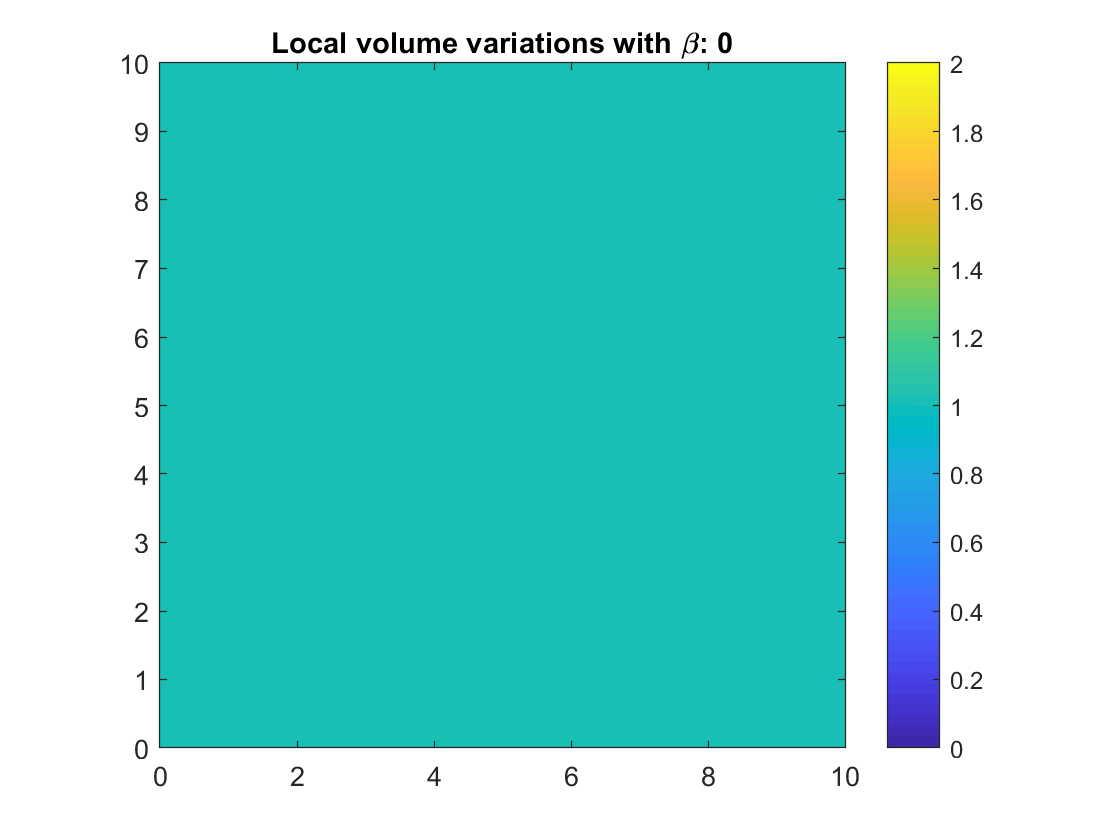
\includegraphics[width=.45\textwidth]{2.png}}\quad
	\subfloat[][$\beta=0.01$]{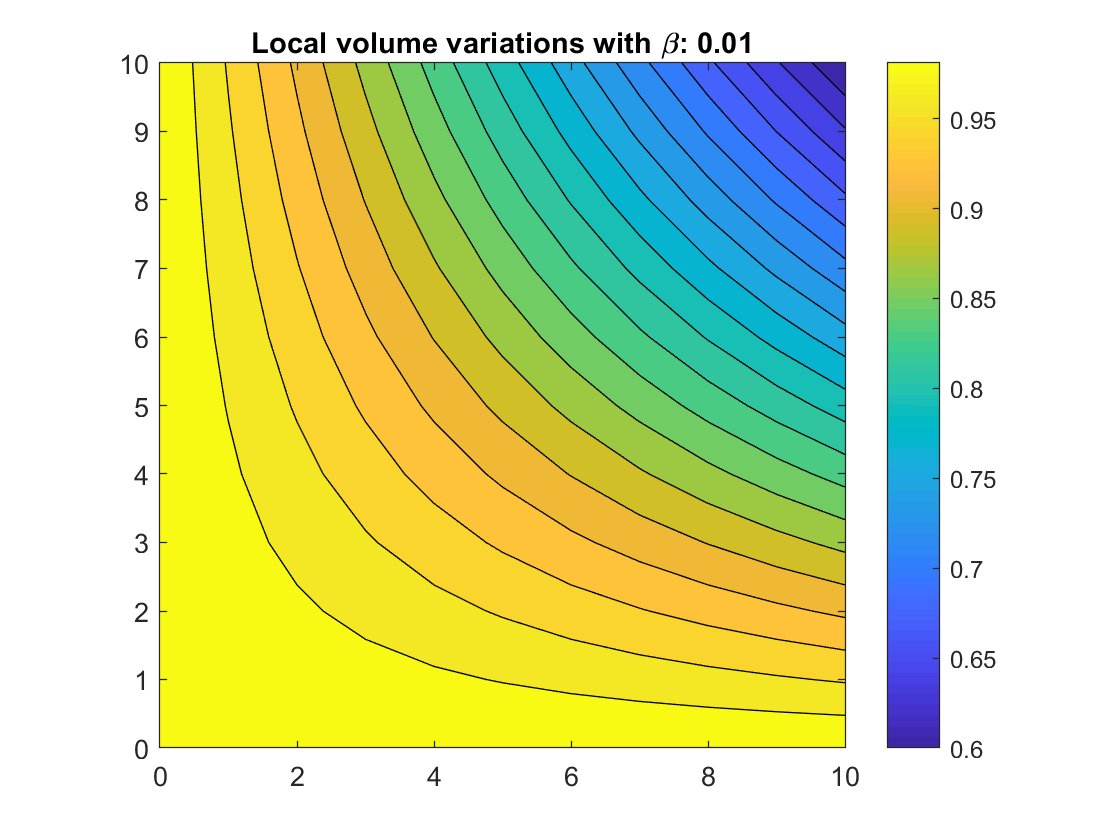
\includegraphics[width=.45\textwidth]{3.png}}\\
	\subfloat[][$\beta=0.025$]{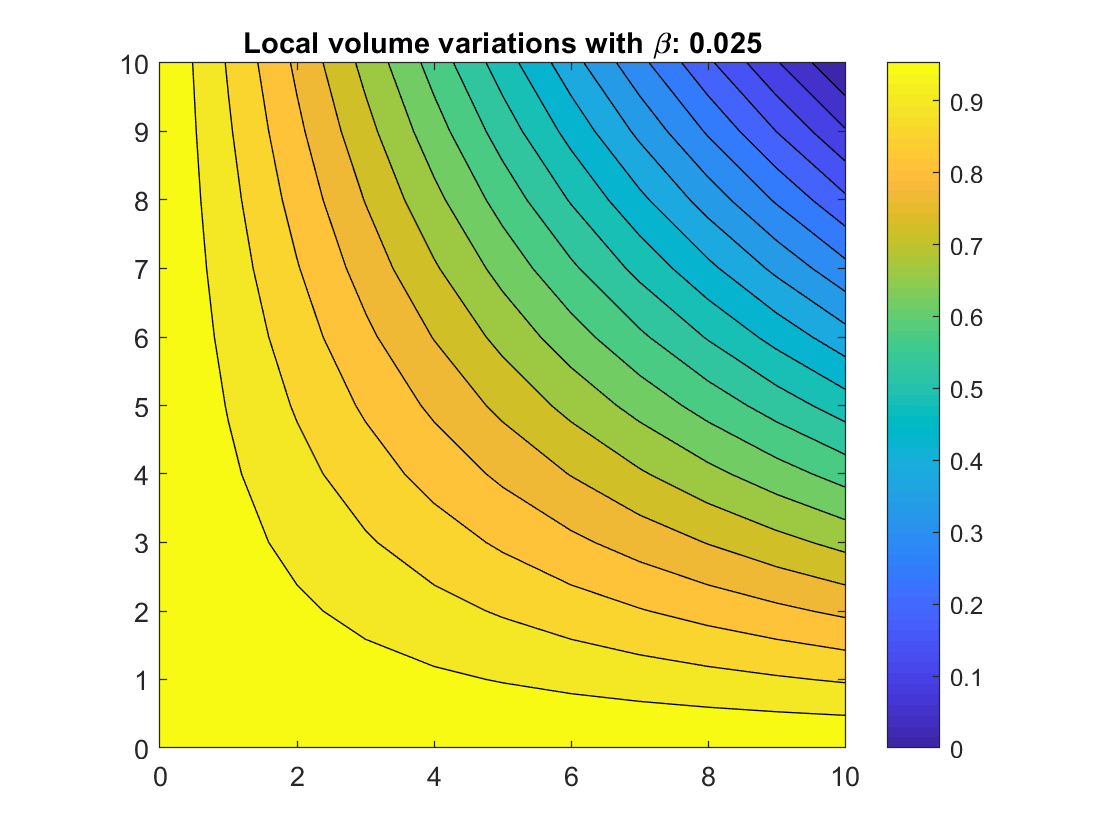
\includegraphics[width=.45\textwidth]{5.png}}\quad
	\subfloat[][$\beta=0.05$]{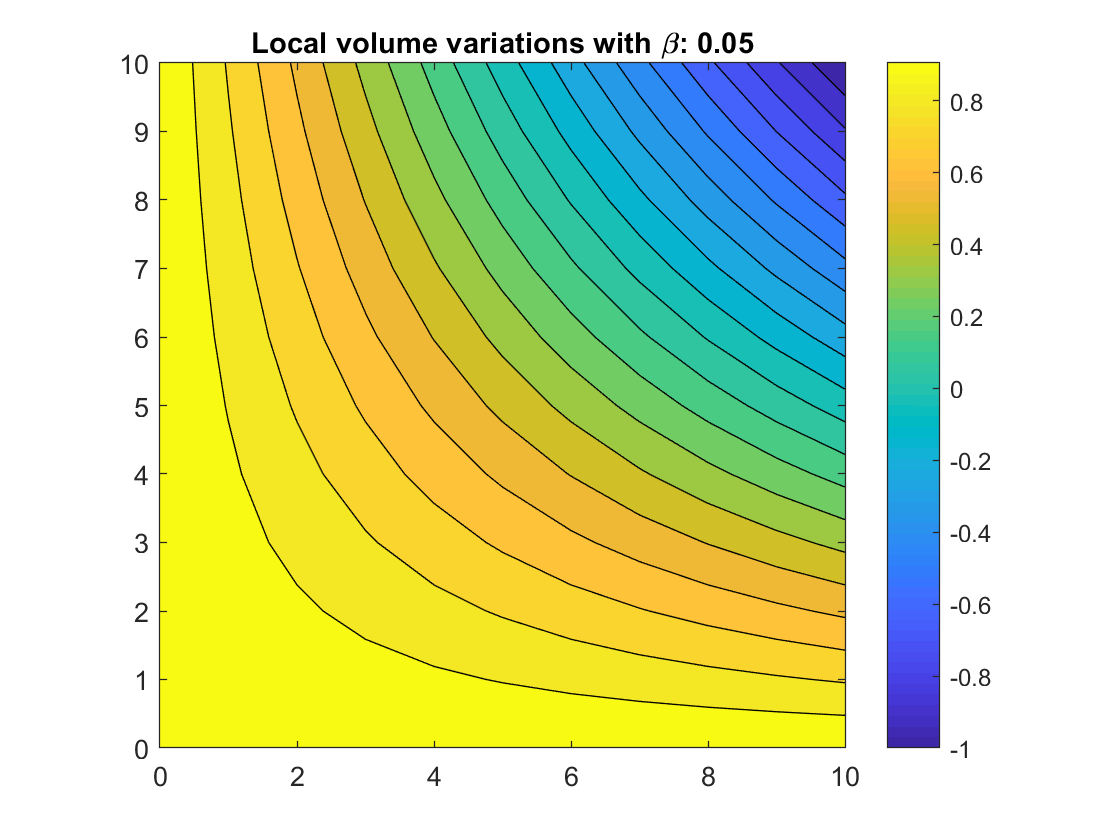
\includegraphics[width=.45\textwidth]{7.png}}
	\caption{Local variation of volume with different $\beta$.}
	\label{fig:3}
\end{figure}

\newpage
\newpage
\noindent \textbf{Question 4:} What is the maximum admissible value for $\beta$ so the transformation has any physical sense? \\

\noindent \textbf{Answer 4:} To make the transformation physical sounds, the determinant of $\underline{\underline{F}}$ should be larger than zero. Otherwise, the deformed volume will be negative, which doesn't make sense. \\
	
	\begin{equation}
	\left| \underline{\underline{F}} \right|=1-0.4\beta {{x}_{1}}{{x}_{2}}>0
	\end{equation}
	Thus,
	\begin{equation}
	\beta {{x}_{1}}{{x}_{2}}<2.5
	\end{equation}
	and also, $\max \left( {{x}_{1}}{{x}_{2}} \right)=100$ in our case. So $\beta$ should satisfy:
	\begin{equation}
	\beta <0.025
	\end{equation}
	
	That's why when choose $\beta=0.05$, there is some region that the local variation of volume is less than zero.
	

	





\end{document}